\documentclass[10pt,a4paper]{article} 
%\documentclass[10pt,a4paper,twocolumn]{article} 

% preamble
%\usepackage{multicol}
\usepackage[pdftex]{graphicx}
\usepackage[T1]{fontenc} 
%\usepackage{fouriernc}
%\usepackage{mathtools}
\usepackage{amsfonts,amsmath,amssymb,amsthm} 
\usepackage[a4paper, hmargin={2.5cm,2.5cm}, vmargin={2.5cm,2.5cm}]{geometry} 
% ------------------------
\usepackage{multicol} % to switch between 1, 1-2, n multicolumn mode
\usepackage{chngcntr} % reset footnote for each chapter
\usepackage{fancyhdr} % headline
\usepackage{enumerate}
\usepackage{wasysym} % symbols
\usepackage{faktor}%for factor rings 
\usepackage{ marvosym }
\usepackage{ragged2e}
\usepackage{blindtext}
%\usepackage{algorithmic}
\usepackage{algorithm}
\usepackage{algpseudocode}
\usepackage{listings}
\usepackage{newclude}   % include() files without auto pagebreak
\usepackage{xcolor}     % for color coding
\usepackage{nameref}    % reference lslistings based on the option [label=]
% -----
\usepackage[sorting=none]{biblatex} %Imports biblatex package, sort references according to appearance in text
\addbibresource{syssec.bib} %Import the bibliography file

% --- lslistings style ---

\definecolor{codegreen}{rgb}{0,0.6,0}
\definecolor{codegray}{rgb}{0.5,0.5,0.5}
\definecolor{codepurple}{rgb}{0.58,0,0.82}
\definecolor{backcolour}{rgb}{0.95,0.95,0.92}
\definecolor{verde}{rgb}{0.25,0.5,0.35}
\definecolor{jpurple}{rgb}{0.5,0,0.35}

\lstdefinestyle{mystyle}{
    backgroundcolor=\color{backcolour},   
    commentstyle=\color{codegreen},
    keywordstyle=\color{magenta},
    numberstyle=\tiny\color{codegray},
    stringstyle=\color{codepurple},
    basicstyle=\ttfamily\footnotesize,
    breakatwhitespace=false,         
    breaklines=true,                 
    captionpos=b,                    
    keepspaces=true,                 
    numbers=left,                    
    numbersep=5pt,                  
    showspaces=false,                
    showstringspaces=false,
    showtabs=false,                  
    tabsize=2
}

\lstset{style=mystyle}

% Coverpage setup
\title{ Systems Security (F25.520212U009.A) \\
        Project 01 \\
        Group 5 \\
        Aarhus University%
}

\author{Miklos Daniel Vadasz}


\begin{document}

\maketitle\thispagestyle{empty}
\makeatletter

\newpage
\tableofcontents\thispagestyle{empty}
\lstlistoflistings
\listofalgorithms
\newpage

% Abastract for RSA-OAEP
\thispagestyle{empty}
\begin{abstract}
    Textbook RSA encryption is not secure. An attacker is able to obtain
ciphertexts for messages that were never encrypted as such.
To prevent such attacks, padding schemes can be used. One such scheme is
standardized as PKCS 1.5, but it suffers from parity and padding oracles in
case the plaintext is not handled properly. A more secure alternative is
OAEP (Optimal Asymmetric Encryption Padding).

In this assignment I made an implementation of the RSA-OAEP according
to [RFC8017] using SHA-256 as hash and mask generation function and an empty label string.

Throughout the implementation I was paying attention to  support for the key generation,
encryption and decryption operations, such that the resulting
cryptosystem is consistent and able to decrypt its own ciphertexts.

Furthermore I choosed the target security level of 128 bits (use RSA moduli of size 3072 bits),
in accirdance  for the selection of  the random number generator for key generation, 
as to avoid the pitfalls discussed in class. 

\end{abstract}

\newpage

% introduction: overview of RSA-OAEP
\setcounter{page}{1}
\section{Introduction}
% Review of RSA-OAEP
% Ide toviden az alapot
Textbook RSA encryption is not secure. An attacker is able to obtain ciphertexts for messages that were never encrypted as such. To prevent such attacks, padding schemes can be used. One such scheme is standardized as PKCS 1.5, but it suffers from parity and padding oracles in case the plaintext is not handled properly. A more secure alternative is OAEP (Optimal Asymmetric Encryption Padding) algorithm which is a form of Feistel Network which uses  random oracles $\mathcal{G}, \mathcal{H}$ prior to asymetric encryption. \cite{Damgaard2025,Bellare1995,Paillier2006,Kilian2001}
 Within the Random Oracle model, combined with secure one-way trapdoor function $f$ this hybrid scheme yields us   a semantically secure scheme under choosen plaintext attack, while combining it with RSA as a result OAEP is proven to be  secure against chosen ciphertext attack.\cite{Damgaard2025,Bellare1995,Paillier2006,Kilian2001}
 
Generally speaking OAEP is a method for turning public-key system with only deterministic security int oa chosen ciphertext secure scheme. \cite{Damgaard2025,Bellare1995,Paillier2006,Kilian2001}

The part of the assignment showcases the implementation of the RSA-OAEP according to RFC8017 \cite{rfc8017} using SHA-256 as hash and mask generation function and an empty label string. In the implementation, the target security level was RSA moduli of size 3072 bits in conjunction with the high-level programming language Python, for its native support for arbitrary-precision integers, byte strings, and its extensive standard library, especially \cite{pyhashlib}.

For the sake of transparency , I used snippets from the most popular forums and code-sharing portals (e.g. \url{stackoverflow.com}, \url{github}) in addition to the referenced literature to solve the assignment. 


% Task 6: Implementing RSA-OEAP

%Textbook RSA encryption is not secure. An attacker is able to obtain ciphertexts for messages that were never encrypted as such. To prevent such attacks, padding schemes can be used. One such scheme is standardized as PKCS 1.5, but it suffers from parity and padding oracles in case the plaintext is not handled properly. A more secure alternative is OAEP (Optimal Asymmetric Encryption Padding).

%The part of the assignment requires the implementation of the RSA-OAEP according to RFC8017 using SHA-256 as hash and mask generation function and an empty label string.

%The objective of this assignment is to implement support for the key generation, encryption and decryption operations, such that the resulting cryptosystem is consistent and able to decrypt its own ciphertexts.

%In your implementation, you should target a security level of 128 bits, i.e., use RSA moduli of size 3072 bits. You are allowed to use library functions such as random number generators and mathematical subroutines (of course you cannot just wrap an existing library for RSA), but you need to document and justify you decisions with respect to security. Especially, be careful when selecting the random number generator for key generation, as to avoid the pitfalls discussed in class. If encoding/decoding presents a challenge, you can reuse existing code as well, or read the IEEE P1363 specification for reference. For reference, the Wikipedia has some good pictures of the RSA-OAEP encoding/decoding functions.

%Any high-level programming language will suffice. Immediate suggestions are Python, for its native support for arbitrary-precision integers, byte strings, and its extensive standard library; Java, due to its library support for multi-precision integers; or the combination of the C programming language with the GMP library.


% ---------------------------------------

\section{Review the Theoretical Background of RSA-OAEP}

\subsection{Overview of the Random Oracle Model for Public-key Cryptosystem}

We say that $(G,E,D)$ Cryptosystem is \textit{chosen ciphertext} ($CCA$) secure, if for all probabilistic polynomial time adversaries (denoted as $PPT$ furthermore) $\mathcal{A}$ the following  condition holds: 
$Adv_{\mathcal{A}} (O_{Real}, O_{ideal}) $ is negligible in $k$, where $G$ denotes the key-generation function , $E$ denotes the encryption function, while $D$ denotes the decryption function respectively.\cite{Damgaard2025}

Let the $G$ key generation \textit{algorithm (\ref{alg:cca-keygen})}  be probabilistic, than for input $k$ (the so called \textit{security parameter})  it always outputs a pair of $p_k$ private key and $s_k$ secret key.\cite{Damgaard2025}


\begin{algorithm}
\caption{Key Generation \(G(k)\)}
\begin{algorithmic}[1]
\State \textbf{Input:} Security parameter \(k\)
\State \textbf{Output:}  Pair of $p_k$ private key and $s_k$ secret key
\State \(p_k, s_k \gets G(k)\) key generation
\State \Return \((p_k, s_k)\)
\end{algorithmic}
\label{alg:cca-keygen}
\end{algorithm}

The encryption algorithm $E$ \textit{(algorithm \ref{alg:cca-enc})}, which is may be probabilistic takes the input $p_k$ and plaintext $x \in \mathcal{P}$, where $\mathcal{P}$ denotes the plaintext space, than produces the output ciphertext: $E_{p_k}(x) \in \mathcal{C}$, where $ \mathcal{C}$ denotes the ciphetext space. \cite{Damgaard2025}

\begin{algorithm}
\caption{Encryption \(E_{p_k}(x)\)}
\begin{algorithmic}[1]
\State \textbf{Input:} Public key \(p_k\), plaintext \(x \in \mathcal{P}\)
\State \textbf{Output:} Ciphertext \(y \in \mathcal{C}\)
\State \(y \gets \text{Encryption of plaintext using } p_k\)
\State \Return \(y\)
\end{algorithmic}\label{alg:cca-enc}
\end{algorithm}


In case of decryption the algorithm $D$ \textit{( algorithm \ref{alg:cca-decryption})} takes as input the secret key $s_k$ and $y \in \mathcal{C}$ ciphertext, than produeces the plaintext as output, consequently it is required for every public-key cryptosystem $\forall x\in \mathcal{P}: x = D_{s_k}(E_{p_k}(x))$ for any key pair $(p_k, s_k)$ generated by $G$.\cite{Damgaard2025}

\begin{algorithm}
\caption{Decryption \(D_{s_k}(y)\)}
\begin{algorithmic}[1]
\State \textbf{Input:} Secret key \(s_k\), ciphertext \(y \in \mathcal{C}\)
\State \textbf{Output:} Plaintext \(x \in \mathcal{P}\)
\State \(x \gets \text{Decryption of ciphertext using } s_k\)
\State \Return \(x\)
\end{algorithmic}
\label{alg:cca-decryption}
\end{algorithm}


The \textit{Distinguishing Advantage} for the adversary
$\mathcal{A}$ can be defined by the \textit{advantage} with an algorithm  can distinguish between two oracles:  Assume that the probabilistic algorithm $\mathcal{A}$  that runs, will have access to either oracle $O_1$ or $O_2$, let $p( \mathcal{A},0)$ be the probability that $\mathcal{A}$ outputs $1$, when talking to $O_0$, and $p( \mathcal{A},1)$ be the probability that $\mathcal{A}$ outputs $1$, when it's talking to $O_1$ consequently.\cite{Damgaard2025}

Now, the advantage of $\mathcal{A}$ regarding the 
distinguishability $O_0$ from $O_1$ is defined by:

\begin{equation}
    Adv_{\mathcal{A}} \left( O_0, O_1\right) = 
    \lvert p(\mathcal{A}, 0)- p(\mathcal{A}, 1) \rvert 
\end{equation}

In case when  the advantage $Adv_{\mathcal{A}} \left( O_0, O_1\right)$ is very small (close to $0$), then it implies that the adversary $\mathcal{A}$ has almost no idea of which oracle he talks to (ideal, real). \cite{Damgaard2025}

As for the \textit{ideal world} case we can think of it as follows: 
    Let $k$ security parameter  be the input for both adversary $\mathcal{A}$ and oracle $O_{ideal}$. Then the oracle runs $G(k)$ to produces the keypair $(p_k, s_k)$ and gives $p_k$ to $\mathcal{A}$. 
    As a next step $\mathcal{A}$ computes a plaintext $x \in \mathcal{P}$ and gives it to $O_{ideal}$ which returns $E_{p_k}(r)$ to $\mathcal{A}$ in response, where $r$ is randomly chosen in $\mathcal{P}$ of the same length as $x$.  In the last step $\mathcal{A}$ outputs a bit $b$.\cite{Damgaard2025}

While, for the \textit{real world} case we can think of follows: 
Let $k$ security parameter  be the input for both adversary $\mathcal{A}$ and oracle $O_{ideal}$. Then the oracle runs $G(k)$ to produces the keypair $(p_k, s_k)$ and gives $p_k$ to $\mathcal{A}$. 
    As a next step $\mathcal{A}$ computes a plaintext $x \in \mathcal{P}$ and gives it to $O_{ideal}$ which returns $E_{p_k}(r)$ to $\mathcal{A}$ in response, where $r$ is randomly chosen in $\mathcal{P}$ of the same length as $x$. In the last step $\mathcal{A}$ outputs a bit $b$.\cite{Damgaard2025}

% --- START::Pseudocode test for cryptoblock drawing ---

% --- END::Pseudocode test for cryptoblock drawing ---

% 
 We say that $(\mathcal{G}, \mathcal{E}, \mathcal{D})$ is \textit{CPA} (\textit{choosen plaintext}) secure (or \textit{semantically secure}) if $\forall PPT\quad \mathcal{A}$ adversaries it holds that $Adv_{\mathcal{A}} \left( O_{real}, O_{ideal}\right)$ is negligible in $k$.\cite{Damgaard2025}

We can do similarly in case of \textit{Chosen Ciphertext Security} ( noted as $CPA$ furthermore ), which model against a passive adversary. \cite{Damgaard2025}

% pp. 106 
As for the \textit{ideal world} case we can think of follows: 
    Let $k$ security parameter  be the input for both adversary $\mathcal{A}$ and oracle $O_{ideal}$. Then the  oracle $O_{ideal}$ runs $G(k)$ to produce $(p_k, s_k)$ and gives $p_k$ to $\mathcal{A}$.\cite{Damgaard2025} 
    As for the second step, the $\mathcal{A}$ adversary is allowed to submit as many $y$ input string to $O_{ideal}$, which will return ${D}_{s_k}(y)$ to $\mathcal{A}$. \cite{Damgaard2025} 
    Thirdly, the adversary $\mathcal{A}$ computes a plaintext $x \in \mathcal{P}$ than gives it to the oracle $O_{ideal}$, which responds with $y_0 = E_{p_k}(r)$, where $r$ is     randomly chosen from $\mathcal{P}$ with the same length as $x$.\cite{Damgaard2025}
    As a forth step $\mathcal{A}$ submit an input string to the oracle with the restriction $y \neq y_0$ as many times as he wants, which will return $D_{s_k}(y)$ to $\mathcal{A}$.  In the last step $\mathcal{A}$ outputs a bit $b$.\cite{Damgaard2025}
As for the \textit{real world} case we can think of follows: 
    Let $k$ security parameter  be the input for both adversary $\mathcal{A}$ and oracle $O_{real}$. Then the  oracle $O_{real}$ runs $G(k)$ to produce $(p_k, s_k)$ and gives $p_k$ to $\mathcal{A}$.\cite{Damgaard2025}
    As for the second step, the $\mathcal{A}$ adversary is allowed to submit as many $y$ input string to $O_{real}$, which will return ${D}_{s_k}(y)$ to $\mathcal{A}$. \cite{Damgaard2025}
    Thirdly, the adversary $\mathcal{A}$ computes a plaintext $x \in \mathcal{P}$ than gives it to the oracle $O_{ideal}$, which responds with $y_0 = E_{p_k}(x)$.\cite{Damgaard2025}
    As a forth step $\mathcal{A}$ submit an input string to the oracle with the restriction $y \neq y_0$ as many times as he wants, which will return $D_{s_k}(y)$ to $\mathcal{A}$.  In the last step $\mathcal{A}$ outputs a bit $b$.\cite{Damgaard2025}

\subsection{Overview of OAEP-based Encryption}

In the preliminary phase, let's assume that the original encryption $E_{p_k}(\cdot)$ works on $k$-bit strings. As a second step we choose $k_0, k_1$ parameters with regards to $k_0 + k_1 < k$ inequality. \cite{Damgaard2025}

With the use of $\mathcal{G}, \mathcal{H}$ cryptographic hash functions (one-way functions, that produces random looking output), the scheme can encrypt messages witn $n$ bits, where $n=k-k_0-k_1$, 
where $\mathcal{G}:\{0,1\}^{k_0} \rightarrow \{0,1\}^{n+k_1}$ and 
$\mathcal{H}: \{0,1\}^{n+k_1} \rightarrow \{ 0,1\}^{k_0} $.

Then, the encryption of message $m$ as follows:

\begin{algorithm}
\caption{OAEP-based Encryption (Overview)}
\begin{algorithmic}[1]
\State \textbf{Input:} \(r \in \{0,1\}^{k_0} \) at random
\State \textbf{Compute:} \(s = \mathcal{G}(r) \oplus (m || 0^{k_1}) \), 
                         \( t = \mathcal{H}(s) \oplus r, w = s||t \)
\State \Return  ciphertext \( E_{p_k}(w) \)
\end{algorithmic}
\end{algorithm}

When it comes to the decryption, one is able to use the $s_k$ secret key to reconstruct $w$, hence $(s,t)$ in case the ciphertext was \textit{legal}. Then we are able to reconstruct $r=t \oplus \mathcal{H}$, consequently $s \oplus G(r)$ should be some $n$-bit string $m$ followed by $k_1$ zeroes.
if that is not the case, then we know that the ciphertext was illegal and as a return we should get an error, otherwise the output: $m$. \cite{Damgaard2025} 

% Ide a 3-540bol a par sort az alapveto problemakrol illetve
% a hivatkozasoakt atemelni a bib-be

\subsection{Review the Underlying Problems with OAEP}

% a javitott valtozatott ide a wiki-rol + a forrasokat beemelni ide
% a kepet is atemelni  a ikirol, ha tulmegy az oldalon akkor 
% a pubkey cryptosystem menjen az aux-ba behivatkozva
% a hash fuggveny valaszttasrol + a masking algoritmusrol 
% a ikirol + a forras -> avi jegyzetbol csak emlitesvolt ide nem kell !

In the original description of OAEP \cite{Bellare1995} with consideration the permutation $f \{0,1\}^{n+k_1} \times \{0,1\}^{k_0} \rightarrow {0,1}^{n+k_1} \times {0,1}^{k_0}$, where $k = n+k_0 + k_1$ it is only required that $f$ is a trapdoor one-way permutation.

However in their paper  \cite{Kilian2001} Eiichiro Fujisaki et. al were also considering two additional related problems with partial-domain one-wayness and the set pertial-domain one-wayness of permutation $f$. $(\tau, \epsilon)$-One-Wayness of $f$ means that for any adversary $\mathcal{A}$ whose running time is bounded by $\tau$ the success probability is formulated as $\mathrm{Succ}^{ow}(\mathcal{A}) = Pr_{s,t} \left[ \mathcal{A}(f(s,t)) = (s,t) \right] $.

In case of $(\tau, \epsilon)$-Partial-Domain One-Wayness of $f$, 
we can think about the following: Any adversary $\mathcal{A}$ whose running time is bounded by $\tau$, calculated as $\mathrm{Succ}^{pd-ow} (\mathcal{A}) = Pr_{s,t}  \left[ \mathcal{A}(f(s,t)=s) \right]$ where the success probability is upper-bounded by $\epsilon$.\cite{Kilian2001} 

Lastly. when the adversary $\mathcal{A}$ that outputs a set of $l$ elements within the time bound $\tau$ with $\epsilon$ upper-bounded probability $\mathrm{Succ}^{s-pd-ow}(\mathcal{A}) = Pr_{s,t} \left[  s \in \mathcal{A}(f(s,t)) \right]$ success probability, called as $(l,\tau, \epsilon)$-Set Partial-Domain One-Wayness of $f$.\cite{Kilian2001}

Within their paper Eiichiro Fujisaki et. al\cite{Kilian2001} showed that the following inequality holds: $\mathrm{Succ}^{pd-ow}(\tau) \geq \mathrm{Succ}^{s-pd-ow}(l,\tau)/l$. They also showed, that for specific choices of $f$ more, efficient reductions may exists. Also in some cases, al three problems written above are polynomially equivalent, which is the case for the chosen RSA permutation, also they proved that the scheme is IND-CCA2 secure in the random oracle model relative to the partial-domain wayness of function $f$ \cite{Bellare1993,Kilian2001, RSA78}.

Within his work Shoup improved the scheme (called OAEP+ ) that works with any trapdoor one-way permutation.  In more recent works it has shown that within the standard model (hash functions $\mathcal{G},\mathcal{H} $ are not modeled as random oracles) it is impossible to prove the IND-CCA2 security of RSA-OAEP under the RSA assumption. \cite{Shoup2001, Paillier2006, Brown2006}

% ------------------------
% The OAEP v2.2 
\section{Implementation of OAEP schema according to RFC 8017}

For implementation purpose I choosed the programming language Python (version number 3.12.8). 
 Please refer to Appendix \ref{app:env-setup} for the environment setup.

\subsection{OAEP Building Blocks}

According to RFC 8017 we have the following bulding blocks for OAEP ( the process for encoding is shown in figure \ref{fig:oaep}) \cite{rfc8017}:

$MGF$ is the Mask generation function , usually \textbf{MGF1}\cite{nistsp2015,rfc8017}, $Hash$ is the chosen Cryptographic hash function ( here I used SHA256 ),
$hLen$ is the length of the output of the hash function in bytes,  $k$ is the security parameter (length of the RSA modulus $n$ in bytes),
$M$ is the message to be padded, with length $mLen$ (at most $ mLen= k - 2 \cdot hLen - 2 $ bytes), $L$ is an optional label to be associated with the message (the label is the empty string by default and can be used to authenticate data without requiring encryption), $PS$ is a byte string of $ k - mLen - 2 \cdot hLen - 2$ null-bytes, lastly $\oplus$ denotes the XOR operation.\cite{wiki2025}

\begin{figure}[h!]
    \centering
    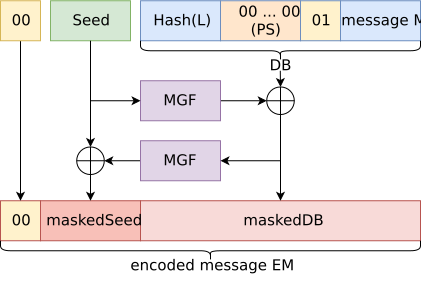
\includegraphics[scale=.65]{OAEP.png}\label{fig:oaep}
    \caption{OAEP encoding schema according to RFC 8017}
    \label{fig:oaep}
\end{figure}

\subsection{OAEP Encoding Scheme}
I implemented the following algorithm for encoding in accordance for PKCS\#1 v2.2 specified OAEP scheme \cite{rfc8017} using the desciption in \cite{wiki2025}.

\begin{algorithm}
\caption{OAEP Encoding Scheme}
\begin{algorithmic}[1]
\State \textbf{Input:} Message $M$, label $L$, hash function $\mathrm{Hash}$, modulus length $k$, and hash length $hLen$
\State \textbf{Output:} Encoded message $\mathrm{EM}$
\State 1. Hash the label $L$ using the chosen SHA256 hash function: $\mathrm{lHash} = \mathrm{Hash}(L)$
\State 2. Generate a padding string $PS$ consisting of $k - \mathrm{mLen} - 2 \cdot \mathrm{hLen} - 2$ bytes with the value 0x00.
\State 3. Concatenate $lHash$, $PS$, the single byte 0x01, and the message $M$ to form a data block $DB$: $\mathrm{DB} = \mathrm{lHash} || \mathrm{PS} || \mathrm{0x01} || \mathrm{M}$. This data block has length $k - \mathrm{hLen} - 1$ bytes.
\State 4. Generate a random seed of length $hLen$. 
\State 5. Use the mask generating function to generate a mask of the appropriate length for the data block: $\mathrm{dbMask} = \mathrm{MGF}(\mathrm{seed}, k - \mathrm{hLen} - 1)$
\State 6. Mask the data block with the generated mask: $\mathrm{maskedDB} = \mathrm{DB} \oplus \mathrm{dbMask}$
\State 7. Use the mask generating function to generate a mask of length $hLen$ for the seed: $\mathrm{seedMask} = \mathrm{MGF}(\mathrm{maskedDB}, \mathrm{hLen})$
\State 8. Mask the seed with the generated mask: $\mathrm{maskedSeed} = \mathrm{seed} \oplus \mathrm{seedMask}$
\State 9. The encoded (padded) message is the byte 0x00 concatenated with the $maskedSeed$ and $maskedDB$: $\mathrm{EM} = \mathrm{0x00} || \mathrm{maskedSeed} || \mathrm{maskedDB}$
\end{algorithmic}
\label{alg:oaep-enc}    
\end{algorithm}

In accordance with \cite{Brown2019,cryptoeprint:2004/304} and using the lecture materials to avoid the pitfalls discussed in class, I choosed SHA256 hashing algorithm  as shown in the Python code snippet (\textit{\nameref{code:hashing}})   from \textit{hashlib} \cite{pyhashlib} instead of SHA-1.


\begin{center}
    \begin{lstlisting}[language=Python,caption=hashlib.sha256(), label=code:hashing]
# ..

def oaep_encode(message, n, e, label=b""):
    # `lHash` labelling using sha256
    lHash = hashlib.sha256(label).digest()
    # ..
    hLen = hashlib.sha256().digest_size  # Hash length for SHA256 -> 32 bytes
# ..

\end{lstlisting}
\end{center}

In accordance to \cite{kernelrandom7, kernelurandom4} and using the lecture materials to avoid the pitfalls discussed in class, Since I'm using Linux I choosed to use \textit{/dev/urandom} as an entropy collector instead of \textit{/dev/random} as shown in the Python code snippet (\textit{\nameref{code:seeding}}). 

In Unix-like operating systems, \textit{/dev/random} and \textit{/dev/urandom} are special files that serve as cryptographically secure pseudorandom number generators (CSPRNGs). They allow access to a CSPRNG that is seeded with entropy (a value that provides randomness) from environmental noise, collected from device drivers and other sources. \cite{kernelrandom7}. 

\begin{lstlisting}[language=Python,caption=os.urandom(), label=code:seeding]
# ..

seed = os.urandom(hLen)

# ..
\end{lstlisting}


The \textit{/dev/urandom} device typically was never a blocking device, even if the pseudorandom number generator seed was not fully initialized with entropy since boot. Since version 5.17 of the Linux kernel, the random number generator switched from using the SHA-1 cryptographic hash function in the entropy collector to BLAKE2s, a newer, faster and more secure hash function.\cite{kernelrandom7, kernelurandom4,wikirandom,blake}


\subsection{OAEP Decoding Scheme}

I implemented the following algorithm for decoding in accordance for PKCS\#1 v2.2 specified OAEP scheme \cite{rfc8017} using the desciption in \cite{wiki2025}:

\begin{algorithm}
\caption{OAEP Decoding Scheme}
\begin{algorithmic}[1]
\State \textbf{Input:} Encoded message $\mathrm{EM}$, label $L$, modulus length $k$, hash length $hLen$
\State \textbf{Output:} Decoded message $M$
\State 1. Hash the label $L$ using the chosen hash function: $\mathrm{lHash} = \mathrm{Hash}(L)$
\State 2. To reverse step 9 in algorithm (\ref{alg:oaep-enc}), split the encoded message $EM$ into the byte 0x00, the $maskedSeed$ (with length $hLen$) and the $maskedDB$:  $\mathrm{EM} = \mathrm{0x00} || \mathrm{maskedSeed} || \mathrm{maskedDB}$
\State 3. Generate the $seedMask$ which was used to mask the $seed$: $\mathrm{seedMask} = \mathrm{MGF}(\mathrm{maskedDB}, \mathrm{hLen})$
\State 4. To reverse step 8 in algorithm (\ref{alg:oaep-enc}), recover the $seed$ with the $seedMask$: $\mathrm{seed} = \mathrm{maskedSeed} \oplus \mathrm{seedMask}$
\State 5. Generate the $dbMask$ which was used to mask the data block: $\mathrm{dbMask} = \mathrm{MGF}(\mathrm{seed}, k - \mathrm{hLen} - 1)$
\State 6. To reverse step 6 in algorithm (\ref{alg:oaep-enc}), recover the data block $DB:$ $\mathrm{DB} = \mathrm{maskedDB} \oplus \mathrm{dbMask}$
\State 7. To reverse step 3 in algorithm (\ref{alg:oaep-enc}), split the data block into its parts: $\mathrm{DB} = \mathrm{lHash'} || \mathrm{PS} || \mathrm{0x01} || \mathrm{M}$.

\begin{itemize}
\item  Verify that:
    \begin{itemize}
        \item  $lHash$' is equal to the computed $lHash$
        \item  $PS$ only consists of bytes 0x00
        \item  $PS$ and $M$ are separated by the 0x01 byte and
        \item  the first byte of $EM$ is the byte 0x00.
        \item  If any of these conditions aren't met, then the padding is invalid.
    \end{itemize}
\end{itemize}
\end{algorithmic}
\label{alg:oaep-dec}
\end{algorithm}

The encoded message can then be encrypted with RSA. The deterministic property of RSA is now avoided by using the OAEP encoding because the seed is randomly generated and influences the entire encoded message.\cite{wiki2025}

\begin{figure}[h!]
    \centering
    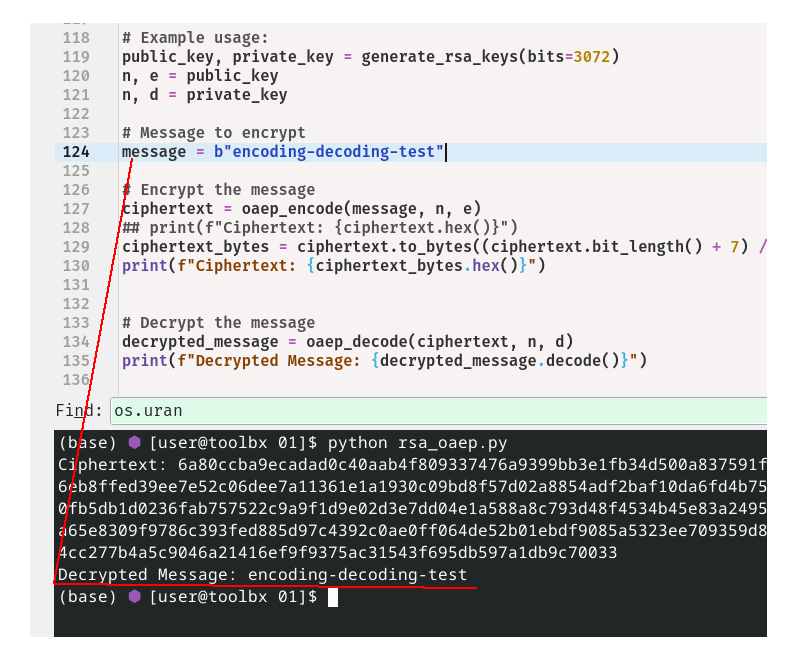
\includegraphics[scale=.5]{02_testrun.png}
    \caption{ Successful testrun with input string: "\textit{encoding-decoding-test}"}
    \label{fig:testrun}
\end{figure}
    
In the PKCS\#1 standard, the random oracles are identical. The \textit{PKCS\#1} standard further requires that the random oracles be \textit{MGF1} with an appropriate hash function.\cite{Brown2019} Last, but not least In figure \textit{\ref{fig:testrun}}, we can observe a succesfull test run by encoding and decoding of input string \textit{encoding-decoding-test}.

\newpage
\printbibliography



\begin{appendix}
\section{Environment Setup on Linux}

As a host environment I use the latest version of Fedora Silverblue (https://docs.fedoraproject.org/en-US/fedora-silverblue/installation/). For interactive command line environment I use Toolbx (\url{https://containertoolbx.org/}), which makes very easy to setup different container environment for development/testing purposes.

\subsection{Create Toolbx Container}

As a base container image I choosed to use Ubuntu (version 24.04).
The installation process can be initiated with the command \lstinline{toolbox create --distro ubuntu --release 24.04 --container $CONTAINER_NAME}, where \lstinline{$CONTAINER_NAME} variable refers to the container's given name.

After pulling the image, we can enter the container with the command \lstinline{$toolbx enter $CONTAINER_NAME}.
Since we were using the latest image the necessary Python version (\lstinline{3.12.X}) package is already installed.

\subsection{Install packages}

The necessary \lstinline{pycrptodome} package can be installed with the command: 
\lstinline{pip install pycryptodome}. 

Further documentation about the installation process can be found at \url{https://pycryptodome.readthedocs.io/en/latest/src/installation.html}.

\subsection{Running the rsa\_oaep.py file}

After changing directory with \lstinline{cd} command to the $\mathrm{rsa\_oaep.py}$ file's location we should be able to run it with the command: \lstinline{python3  rsa_oaep.py}
\label{app:env-setup}
\end{appendix}

\end{document}
